% =====================================================================
\section{Results}\label{sec:results}
% =====================================================================
This section answers the question of Section~\ref{sec:introduction} first on the predeclared held-out comparison (Section~\ref{subsec:heldout}). It then reports the exploratory campaigns that shaped that comparison's policy (Section~\ref{subsec:exploratory}) and additional descriptive analyses of drift and historical variation (Section~\ref{subsec:descriptive}). The experimental unit and what the design cannot identify are stated in Section~\ref{subsec:scope}; held-out and exploratory results are never pooled.

% ---------------------------------------------------------------------
\subsection{The held-out factorial}\label{subsec:heldout}
% ---------------------------------------------------------------------
The held-out campaign asks whether a reserved margin, historical scenarios with activation, or both keep a visit-minimising layout inside the two-sided band on later orders. It deploys the four arms at order index 243,151 and scores each returned layout on the next 21,874 complete orders.

Every comparison with the incumbent layout below carries one asymmetry. The targets $b_s$ are the incumbent's own historical shares \eqref{eq:target}, so the incumbent starts with the whole allowance as headroom, whereas an optimised layout spends it. The incumbent's minimum required slack is 0 on the single history scenario on which NOM and TIGHT train, and about 0.0157 on the scenario set of HIST+ACT and HIST+ACT-T (the 11 historical blocks and the history scenario, with activation), which lies inside $\delta=0.02$ but above the tightened allowance of 0.01. The incumbent is scored on the same window as context, not as a feasibility standard for the optimised arms.

\paragraph{Primary endpoint.} TIGHT satisfied the two-sided band with $\delta=0.02$ on all three optimiser seeds, against a predeclared threshold of two, so the primary endpoint was met. The predeclaration names it the ``Replication endpoint''; it tests the same policy at a later origin of the same order stream, whose history contains the exploratory origin's data. Meeting it supports a bounded case-study claim about this policy at this origin.

\paragraph{Pass pattern and breaches.} The arms that satisfied the band are exactly the arms that reserved a margin: TIGHT and HIST+ACT-T satisfied it on 3/3 seeds, and NOM and HIST+ACT on 0/3 (Table~\ref{tab:heldout_seeds}). This is a two-factor comparison under equal configured solve budgets at one origin; it is not a causal law, and it does not isolate the margin from solver and layout effects. The misses of the two arms without a margin differ in size: the worst breach of HIST+ACT was at most 0.179 percentage points, and that of NOM, the unprotected (0,\,0) control, at least 0.939. NOM missed on both sides of the band on every seed; HIST+ACT missed below the floor on every seed and above the cap on two, and the table gives the counts and magnitudes on each side. A small breach is still a miss of the declared policy. The misses of NOM are reported here as the contrast given by the unprotected control, and those of HIST+ACT are discussed as a limitation in Section~\ref{subsec:limitations}. Figure~\ref{fig:heldout_visits_breach} places the 12 returned layouts by worst breach and visits, and Figure~\ref{fig:heldout_station_shares} shows at which stations each breach occurred.

\begin{table}[htbp]
\centering
\caption{Held-out outcome of each returned layout: origin 243,151, $n=21{,}874$, two-sided band with $\delta=0.02$ over the 24 evaluated stations.}
\label{tab:heldout_seeds}
\small
\setlength{\tabcolsep}{4pt}
\begin{tabular}{@{}llcrrrrrr@{}}
\toprule
 & & & \multicolumn{2}{c}{Above cap} & \multicolumn{2}{c}{Below floor} & Largest & Visits \\
\cmidrule(lr){4-5}\cmidrule(lr){6-7}
Arm & Seed & Band & Stations & Worst & Stations & Worst & deviation & per order \\
\midrule
NOM        & 11 & miss & 4 & 1.006 & 5 & 0.178 & 3.006 & 3.266 \\
           & 22 & miss & 4 & 0.939 & 4 & 0.233 & 2.939 & 3.256 \\
           & 33 & miss & 2 & 1.144 & 4 & 0.167 & 3.144 & 3.172 \\
\addlinespace
TIGHT      & 11 & pass & 0 & 0.000 & 0 & 0.000 & 1.756 & 3.266 \\
           & 22 & pass & 0 & 0.000 & 0 & 0.000 & 1.209 & 3.267 \\
           & 33 & pass & 0 & 0.000 & 0 & 0.000 & 1.357 & 3.276 \\
\addlinespace
HIST+ACT   & 11 & miss & 1 & 0.081 & 1 & 0.039 & 2.081 & 3.278 \\
           & 22 & miss & 2 & 0.085 & 2 & 0.179 & 2.179 & 3.239 \\
           & 33 & miss & 0 & 0.000 & 2 & 0.069 & 2.069 & 3.274 \\
\addlinespace
HIST+ACT-T & 11 & pass & 0 & 0.000 & 0 & 0.000 & 1.026 & 3.351 \\
           & 22 & pass & 0 & 0.000 & 0 & 0.000 & 1.160 & 3.386 \\
           & 33 & pass & 0 & 0.000 & 0 & 0.000 & 1.039 & 3.304 \\
\midrule
Incumbent  &    & pass & 0 & 0.000 & 0 & 0.000 & 1.157 & 3.847 \\
\bottomrule
\end{tabular}
\par\smallskip
\begin{minipage}{\linewidth}\footnotesize
Band: pass when every station's realised share lies in $[\max(0,b_s-\delta),\min(1,b_s+\delta)]$. Stations: number of stations beyond that side of the band. Worst: largest excess beyond it, in percentage points. Largest deviation: largest $|r_s-b_s|$ over the 24 stations, in percentage points. Visits per order: mean future station visits over the window's orders. Arms are defined in Table~\ref{tab:arms}; every optimised layout is time-capped. Incumbent: the site's layout, whose own historical shares define $b_s$, scored on the same window as context.
\end{minipage}
\end{table}

\begin{figure}[htbp]
\centering
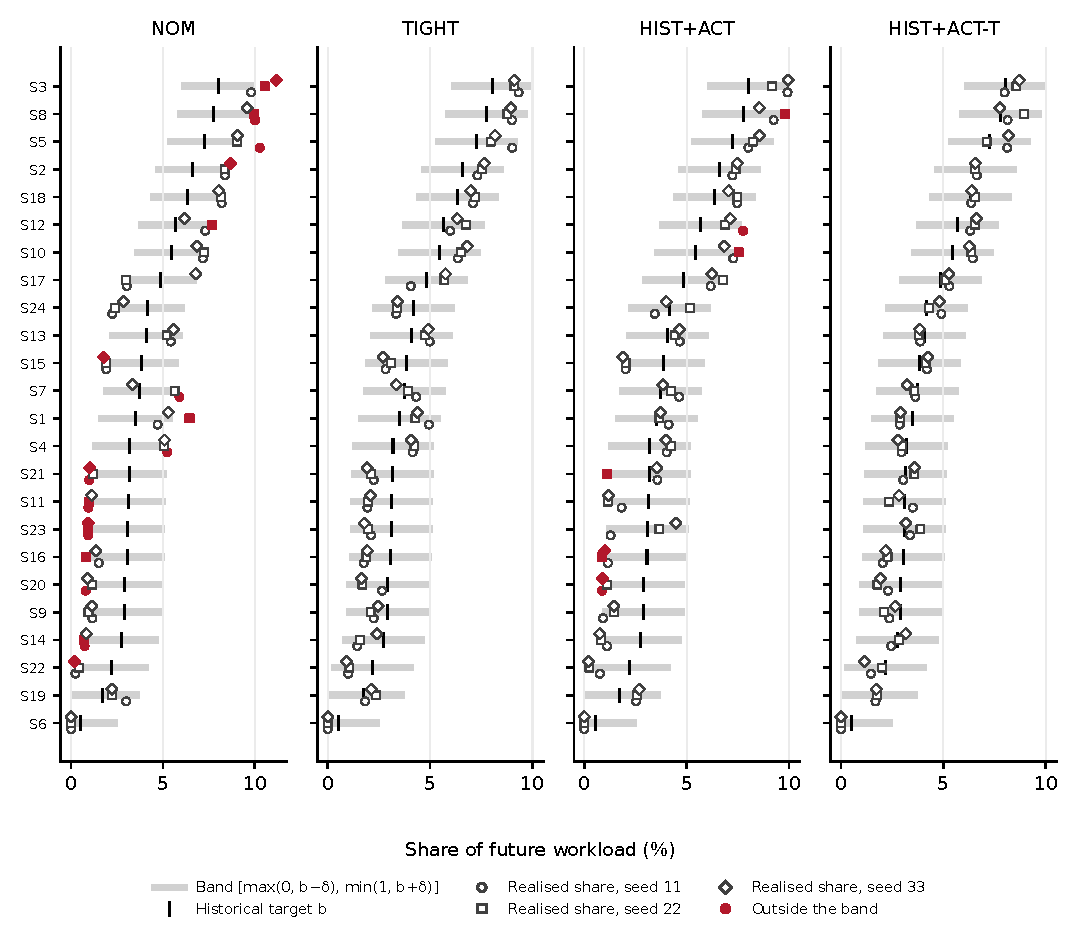
\includegraphics[width=\textwidth]{figures/fig_heldout_station_shares.pdf}
\caption{Realised future workload shares of the 24 evaluated stations on the held-out window (origin 243,151, $n=21{,}874$), one panel per arm. Rows are stations, labelled with the companion's aliases and sorted by historical target $b_s$ (black tick), which is computed on the orders before the origin under the incumbent layout and frozen. The grey bar is the band $[\max(0,b_s-\delta),\min(1,b_s+\delta)]$ with $\delta=0.02$. Markers give the realised share for each optimiser seed and are filled when the share lies outside the band. Shares are in percent.}
\label{fig:heldout_station_shares}
\end{figure}

\paragraph{Deviation from target and visits.} At both margin levels the arm with historical scenarios and activation kept the largest station deviation from target lower than the matching arm without them on every seed, and it had higher mean visits per order (Table~\ref{tab:heldout_arms}). With the margin, HIST+ACT-T kept its largest station deviation between 1.026 and 1.160 percentage points over the seeds, against 1.209 to 1.756 for TIGHT, and made 2.4\% more mean future visits per order than TIGHT; the visit ranges of these two arms do not overlap, whereas those of the two arms without the margin do. The scenario-and-activation arms thus kept the largest station deviation lower at higher mean visits per order; they did not change which arms satisfied the band. Scenarios and activation are bundled in this design, so their separate contributions are not identified, and the deviation comparison and the visit ratio are additional descriptive analyses of time-capped returned layouts. On the maximum-deviation statistic HIST+ACT-T, at most 1.160 over the seeds, is close to the incumbent's 1.157 on the same window; the statistic does not show that their station profiles are the same.

\begin{table}[htbp]
\centering
\caption{Held-out results by arm over three optimiser seeds, with the incumbent layout scored on the same window.}
\label{tab:heldout_arms}
\small
\setlength{\tabcolsep}{4pt}
\begin{tabular}{@{}lcccrc@{}}
\toprule
 & Seeds & \multicolumn{2}{c}{Visits per order} & Saving vs & Largest deviation \\
\cmidrule(lr){3-4}
Arm (scenarios, margin) & in band & Mean & [min, max] & incumbent (\%) & [min, max] (pp) \\
\midrule
NOM (0,\,0)        & 0/3 & 3.232 & [3.172, 3.266] & 16.0 & [2.939, 3.144] \\
TIGHT (0,\,1)      & 3/3 & 3.270 & [3.266, 3.276] & 15.0 & [1.209, 1.756] \\
HIST+ACT (1,\,0)   & 0/3 & 3.264 & [3.239, 3.278] & 15.2 & [2.069, 2.179] \\
HIST+ACT-T (1,\,1) & 3/3 & 3.347 & [3.304, 3.386] & 13.0 & [1.026, 1.160] \\
\midrule
Incumbent          & in band & 3.847 &  & (reference) & 1.157 \\
\bottomrule
\end{tabular}
\par\smallskip
\begin{minipage}{\linewidth}\footnotesize
Mean: arithmetic mean over the three seeds. [min, max]: range over the seeds. Saving: reduction of the arm's mean visits per order against the incumbent's 3.847 on the same window. The incumbent's targets are its own historical shares, so it starts with the whole allowance as headroom. Visits compare time-capped returned layouts, not optima.
\end{minipage}
\end{table}

\paragraph{Visits against the incumbent.} Every optimised arm made fewer visits per order than the incumbent, which made 3.847 on the same window: the arm-level means were 13.0\% to 16.0\% lower, and Table~\ref{tab:heldout_arms} gives each arm's saving next to its pass count. Single runs made 12.0\% to 15.1\% fewer visits for the two margin arms and 14.8\% to 17.5\% fewer for the two arms without a margin, all of them time-capped returned layouts. These savings are not comparable with the companion's figures \citep{belul_companion}. Its 13.7\% is measured in sample over the whole planning horizon rather than on a later window, and under station budget rows rather than a share band. Its 6.6\% and 7.4\% on unseen weeks come from a different dated extract, order stream, reference layout and workload restriction.

\begin{figure}[htbp]
\centering
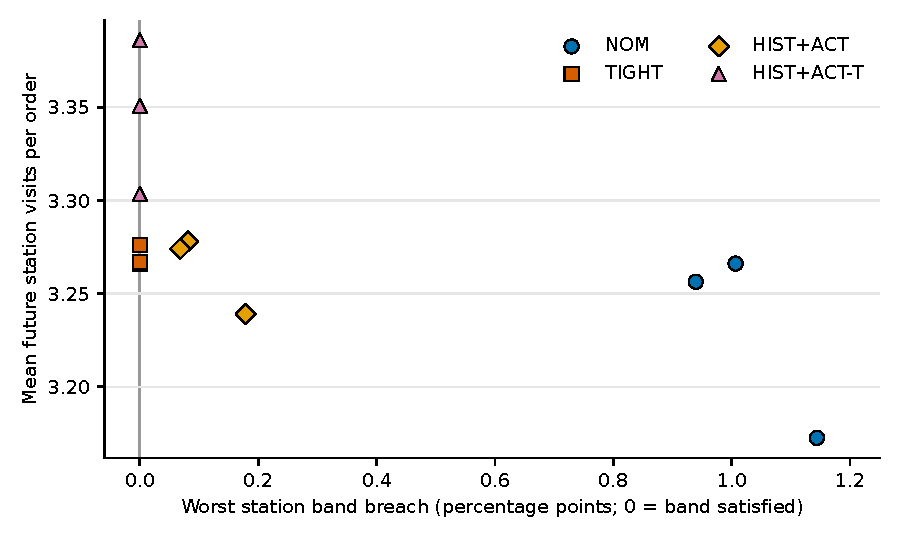
\includegraphics[width=0.85\linewidth]{figures/fig_heldout_visits_breach.pdf}
\caption{Held-out outcomes of the 12 returned layouts (four arms, three optimiser seeds each) at origin 243,151 with $n=21{,}874$: mean future station visits per order against the worst station band breach in percentage points, where 0 means that all 24 evaluated stations satisfied the two-sided band with $\delta=0.02$. Two TIGHT markers nearly coincide. The incumbent layout, which satisfied the band on the same window, made 3.847 visits per order and lies outside the plotted range. Every layout is time-capped, so visit differences compare returned layouts, not optima.}
\label{fig:heldout_visits_breach}
\end{figure}

\paragraph{Training allowance and the modelled set.} Every returned layout used almost exactly the training allowance its arm was given (Table~\ref{tab:heldout_diag}). The layouts without a margin required between 0.019997 and 0.019999 of the allowed 0.02, and the layouts with the margin between 0.009992 and 0.009999 of the allowed $(1-\lambda)\delta=0.01$. These values are measured on each arm's own training set, not on the future window, and they describe time-capped returned layouts; they are additional descriptive analyses.

The realised future lay outside the modelled set of every returned layout, mostly in the downward direction for the scenario arms (Table~\ref{tab:heldout_diag}). For NOM and TIGHT the modelled set is the single pooled-history point, which a station leaves unless its share is unchanged; all 24 stations lay off it on every seed, and those counts are not comparable with the scenario arms' counts. Leaving the modelled set is not a band violation: both margin arms left their sets and still satisfied the band. A departure at one station proves that the future was outside the set, whereas staying inside every station's range would not have proved membership.

\begin{table}[htbp]
\centering
\caption{Training-side diagnostics of the held-out layouts: minimum required slack \eqref{eq:slack} on each arm's own modelled set, and stations whose realised future share lay above or below the range of that set.}
\label{tab:heldout_diag}
\small
\setlength{\tabcolsep}{4pt}
\begin{tabular}{@{}lccccccc@{}}
\toprule
 & Training & \multicolumn{3}{c}{Minimum required slack (share)} & \multicolumn{3}{c}{Stations above / below the set} \\
\cmidrule(lr){3-5}\cmidrule(lr){6-8}
Arm & half-width & Seed 11 & Seed 22 & Seed 33 & Seed 11 & Seed 22 & Seed 33 \\
\midrule
NOM        & 0.02 & 0.019998 & 0.019999 & 0.019999 & 11 / 13 & 11 / 13 & 11 / 13 \\
TIGHT      & 0.01 & 0.009992 & 0.009996 & 0.009999 & 12 / 12 & 11 / 13 & 11 / 13 \\
HIST+ACT   & 0.02 & 0.019997 & 0.019997 & 0.019999 & 1 / 3 & 3 / 4 & 0 / 4 \\
HIST+ACT-T & 0.01 & 0.009993 & 0.009998 & 0.009998 & 0 / 2 & 1 / 4 & 0 / 4 \\
\bottomrule
\end{tabular}
\par\smallskip
\begin{minipage}{\linewidth}\footnotesize
Training half-width: $\delta=0.02$ without a margin and $(1-\lambda)\delta=0.01$ with it. The incumbent's minimum required slack is 0 on the history scenario of NOM and TIGHT and about 0.0157 on the scenario set of HIST+ACT and HIST+ACT-T. For NOM and TIGHT the modelled set is one point, which a station leaves unless its share is unchanged; all 24 lay off it, and their counts are not comparable with those of the scenario arms. Minimum slack is an additional descriptive analysis; departures are a predeclared secondary metric.
\end{minipage}
\end{table}

\paragraph{Solver returns.} All 12 held-out solves returned time-capped layouts with no proof of optimality. Each ended with a relative gap of about 98.5\% against a bound of 11,517 on the training visit objective \eqref{eq:obj}, not on future visits, so the bound gives no evidence that any returned layout is near optimal, and visit differences between arms compare returned layouts under equal configured budgets, not optimal values (Supplementary Section S1).

% ---------------------------------------------------------------------
\subsection{Exploratory context at origin 199,403}\label{subsec:exploratory}
% ---------------------------------------------------------------------
The campaigns in this subsection preceded the held-out factorial and shaped its policy. Each has one optimiser seed at one origin, and its three horizons share that origin, so they are not repeated draws. The two-sided policy was fixed before its solves but after the same futures had been examined under the upper-only rule.

\begin{table}[htbp]
\centering
\caption{Exploratory campaigns on Company~A at origin 199,403 with one optimiser seed: number of the three horizons $n\in\{10{,}937,\ 21{,}874,\ 43{,}748\}$ at which each arm satisfied the rule.}
\label{tab:exploratory}
\small
\begin{tabular}{@{}lccccc@{}}
\toprule
 & Layouts & Upper-only & \multicolumn{3}{c}{Two-sided} \\
\cmidrule(lr){4-6}
Arm & per campaign & $\delta=0.01$ & $\delta=0.01$ & $\delta=0.02$ & $\delta=0.03$ \\
\midrule
NOM      & 1 & 0/3 & 0/3 & 0/3 & 0/3 \\
TIGHT    & 1 & 0/3 & 1/3 & 3/3 & 3/3 \\
HIST     & 3 & 0/3 & 0/3 & 0/3 & 0/3 \\
HIST+ACT & 3 & 2/3 & 0/3 & 1/3 & 0/3 \\
\bottomrule
\end{tabular}
\par\smallskip
\begin{minipage}{\linewidth}\footnotesize
Layouts per campaign: distinct layouts behind the three horizons. NOM and TIGHT train on pooled history, which does not depend on $n$, so one layout is scored three times; HIST and HIST+ACT solve once per horizon, and counts of arms with different layout numbers are therefore not like counts. TIGHT uses $\lambda=0.5$ and the activation arm $\nu=0.01$. Exploratory evidence, never pooled with the held-out results.
\end{minipage}
\end{table}

\paragraph{Upper-only and two-sided rules.} The two rules order TIGHT and HIST+ACT differently (Table~\ref{tab:exploratory}). Under the upper-only rule with $\delta=0.01$, HIST+ACT satisfied the caps at two of the three horizons and NOM, TIGHT and HIST at none. Under the two-sided rule with $\delta=0.02$, TIGHT satisfied the band at all three horizons, HIST+ACT at one, and NOM and HIST at none. These are not like counts: each of NOM and TIGHT contributed one layout scored at three nested horizons, whereas HIST and HIST+ACT contributed three layouts. The different ordering is consistent with the size and side of the margin that each rule reserved for TIGHT. Its layouts required a training allowance of about 0.005 under the upper-only rule, so half a percentage point was reserved, on the cap side only; under the two-sided rule with $\delta=0.02$ they required about 0.010, so one percentage point was reserved on each side. Consistency with the margin size is not a causal isolation, and an upper-only pass limits increases only, so it does not show that station profiles were preserved (Section~\ref{subsec:uncertainty}).

Under the two-sided rule the misses of the scenario arms were mostly, but not only, below the floor: summed over the three horizons, HIST+ACT had 0 cap and 3 floor breaches and HIST 1 cap and 8 floor breaches. In every two-sided cell on Company~A the realised future also fell below the lowest modelled share at some station; leaving the modelled set and breaching the band are different metrics.

\paragraph{Band width.} Each value of $\delta$ is a separately optimised model and a separate solve. With $\delta=0.03$, TIGHT satisfied the band at all three horizons and NOM, HIST and HIST+ACT at none; with $\delta=0.01$, TIGHT satisfied it at one horizon and the other arms at none, with the same layout counts as above. A wider band did not bring the scenario arms into compliance at this origin, and the narrower band was met once. The three values of $\delta$ form a sampled response, not a frontier. No lower bound was certified, so no band is shown to be out of reach, and no $\lambda$ frontier was run.

\paragraph{Synthetic instances.} Synthetic instances enter the exploratory campaigns as a control on finite-sample and solver effects, not as evidence about robustness to drift, because their generator is stationary. Under the two-sided rule they consist of 4 warehouses at one origin with one seed. Their sets of historically inactive products are empty, so HIST+ACT is the same model as HIST on them; that equality is an identity, not evidence that activation protection is costless or beneficial. Under the upper-only rule the larger synthetic screen supports no single ranking of historical scenarios against tightening: the comparison is mixed across catalogue-size strata and rests on unequal scored denominators, because the scenario arms returned no layout within the time limit in part of the smallest family, which is not infeasibility. Supplementary Section S5 reports the synthetic outcomes, including the cells without a returned layout.

% ---------------------------------------------------------------------
\subsection{Additional descriptive analyses: drift, a sufficient margin condition and historical variation}\label{subsec:descriptive}
% ---------------------------------------------------------------------
The analyses in this subsection were not predeclared endpoints. They describe how far the scored windows moved from history and how the reserved margin compares with the site's historical station-level variation. The drift analysis was computed after the held-out window had been scored; the margin was not chosen from it and is not re-chosen after the result.

\begin{table}[htbp]
\centering
\caption{Additional descriptive analyses: total-variation distances of product mixes and the incumbent's historical station-share deviations, against two references.}
\label{tab:context}
\small
\begin{tabular}{@{}p{6.4cm}cc@{}}
\toprule
Quantity & Stored & Like for like \\
\midrule
\multicolumn{3}{@{}p{10.4cm}}{\emph{Total-variation distance from pooled history; history before order index 243,151, blocks of $n=21{,}874$ orders}} \\
Largest of the 11 historical blocks & 0.194 & about 0.214 \\
Held-out window, ex post & 0.195 & not applicable \\
\midrule
\multicolumn{3}{@{}p{10.4cm}}{\emph{Incumbent's largest station-share deviation in one historical block (pp); history before order index 199,403}} \\
$n=10{,}937$ & 1.70 & about 1.80 \\
$n=21{,}874$ & 1.63 & about 1.83 \\
$n=43{,}748$ & 1.47 & about 1.89 \\
\bottomrule
\end{tabular}
\par\smallskip
\begin{minipage}{\linewidth}\footnotesize
Stored: each block measured against a pooled history that contains it. Like for like: against the rest of the history, obtained by dividing the stored value by one minus the block's mass fraction; block line mass is not stored, so the fraction is taken by order count (about 0.09 for the held-out history). The stored mean over the 11 blocks is 0.171. The deviations belong to the incumbent layout and exist only for the exploratory history. None of these values was a predeclared endpoint.
\end{minipage}
\end{table}

\paragraph{Product-mix drift.} Measured against the rest of the history, the largest historical block distance is about 0.214, and the held-out product mix, at a total-variation distance of 0.195 from the pooled history against which it was scored, lies below it (Table~\ref{tab:context}). The stored historical maximum of 0.194 measures each block against a pooled history that contains that block, which shrinks each value by the factor one minus the block's mass fraction (Supplementary Section S6). Block line mass is not stored, so that fraction is taken by order count, about 0.09; the stored ordering reverses for any mass fraction above about 0.0028. The incumbent layout satisfied the two-sided band on the held-out window. Total-variation distance measures change in the product mix, not change in station shares, because changes among the products of one station can cancel in its share.

\paragraph{A sufficient margin condition.} The second proposition of Section~\ref{subsec:conditional} gives a sufficient condition for the margin arms: a layout inside the tightened band on pooled history stays inside the policy band on any future within total-variation distance $\lambda\delta=0.01$ of that history. The condition did not hold on any analysed window. The held-out distance of 0.195 is many times the reserved margin, and the stored distances of the futures scored at the exploratory origin also exceed it. The margin arms nevertheless satisfied the band on every held-out seed, which is consistent with product-level changes cancelling within stations but does not establish it. The failure of a sufficient condition does not establish any particular alternative rule for choosing the margin.

\paragraph{Historical station-level variation and the reserve.} A check of the reserve against the site's historical station-level variation did not predict compliance here. The statistic checked is the incumbent layout's largest station-share deviation in a single historical block on the earlier, exploratory history: 1.63 percentage points at $n=21{,}874$ with each block measured against a pooled history that contains it, and about 1.83 against the rest of the history (Table~\ref{tab:context} gives all three horizons). Under either reference the reserve of one percentage point was smaller, yet both margin arms satisfied the band on every held-out seed. The half-width $\delta=0.02$ was chosen using this statistic, and the reserved margin is $\lambda\delta$; no rule linking the margin to that statistic was tested. The values come from the exploratory history, and none is available for the held-out history. The incumbent's variation belongs to its own layout, so the check informs but does not set the reserve for an optimised layout. No validated rule for choosing the margin was obtained.
